\section{Circuit design and stage-level simulations}
\label{sec:Schematic_Design}
This chapter discusses the chosen topology and its characteristics by presenting the individual stages, their parameters and the main design choices. Then it compares the independently EM-simulated cores to evaluate the deviation from the ideal results. Finally, the ideal and EM versions of the merged cores, without matching networks, are compared.\\
The design aims to realize an active balun supplied from a \SI{1.8}{\volt} source, with amplitude and phase imbalances equal to or lower than $\pm 0.5\,\si{\decibel}$ and $\pm 1^{\circ}$, respectively, while remaining efficient and providing gain over the D-band. Although intended for D-band applications, the results are shown over the \SIrange{100}{200}{\giga\hertz} range to provide a more complete overview of its frequency behavior.\\
The proposed design consists of three stages:
\begin{itemize}
    \item a single input-balanced output differential amplifier;
    \item a differential input-differential output amplifier;
    \item an output amplifier stage.
\end{itemize}

\subsection{Design and analysis at the schematic level}
\subsubsection{Design of the First Stage}
\label{subsubsec:Design of the First Stage}
\begin{figure}[hbt!]
    \centering
    \begin{circuitikz}[scale=0.85, transform shape]
    \draw (0,0) node[npn, xscale=1, anchor=B] (Q1)
    {\shortstack{$Q1$ \\ 2}};
    %metto metà sinistra dell'emettitore
    \draw (Q1.E)--++(0,-0.35)--++(1.1,0) coordinate(e);
    %metto metà destra dell'emettitore e Q2
    \draw(e)--++(1.1,0) --++(0,+0.35) node[npn, xscale=-1, anchor=E] (Q2){\ctikzflipx{\shortstack{$Q2$ \\ 2}}};
    %disegno current mirror
    \draw (e) to [short,*-]++(0,-0.25) node[npn, xscale=1, anchor=C] (Q3)
    {\shortstack{$Q3$ \\ 2}};
    \draw (Q3.E) --++(0,-0.5) node[npn, xscale=1, anchor=C] (Q4){\shortstack{$Q4$ \\ 2}} ;
    \draw (Q4.E) --++(0,-0.15) node[tlground]{};
    
    %inserisco le resistenze bias AC block
    %biasin a Q1
    \draw (Q1.B)--++(-0.85,0) coordinate (in1)
    to [R,l=$\mathrm{R}_1$]++(0,1.5)
    to [open]++(-0.35,0) --  node[anchor=south] {$\mathrm{V}_{\mathrm{CC}}$} ++(0.7,0);
    %biasing a Q2
    \draw (Q2.B)--++(0.85,0) coordinate (in2)
    to [R,l=$\mathrm{R}_2$]++(0,1.5) to [open]++(-0.35,0) --  node[anchor=south] {$\mathrm{V}_{\mathrm{CC}}$} ++(0.7,0);
    %biasing current mirror Q3
    \draw (Q3.B) to [short]++(-0.15,0) coordinate (in3);
    \draw (in3)to [short,*-]++(-0.25,0) to [R,l_=$\mathrm{R}_3$]++(-2,0) to [short,-o]++(-0.25,0) node[left]{$\mathrm{V}_{\mathrm{B2}}$};
    \draw (in3) to [C,l_=$C_{1}$]++(0,-1.25)node[tlground]{};
    %biasing current mirror Q4
    \draw (Q4.B) to [R,l_=$\mathrm{R}_4$]++(-1.25,0) to [short,-o]++(-0.25,0) node[left]{$\mathrm{V}_{\mathrm{B1}}$};
    %inserisco input a base Q1
    \draw (in1) to [C,*-o] ++(-2,0) coordinate(dc1)node[left]{$v_{se}$};
    
    \draw (dc1) to [open]++(0.475,-0.375) rectangle++(1.05,0.75);
    
    %inserisco capacità a base Q2
    \draw (in2)to [open,-*]++(-0.5,0) to [C,l=$C_{2}$]++(0,-1.25)node[ground]{};
    
    %disegno collettore Q1
    \draw (Q1.C) --++ (0,1) coordinate(c1) to [L]++(0,2.15) to [open]++(-0.35,0) --  node[anchor=south] {$\mathrm{V}_{\mathrm{CC}}$} ++(0.7,0);
    \draw (c1) to [short,*-o]++(0.5,0)node[above]{+};
    
    \draw (Q2.C) --++ (0,1) coordinate(c2) to [L]++(0,2.15) to [open]++(-0.35,0) --  node[anchor=south] {$\mathrm{V}_{\mathrm{CC}}$} ++(0.7,0);
    \draw (c2) to [short,*-o]++(-0.5,0)node[above]{-};
    

      \node[draw, fill=white, rounded corners] at (8,2) {
      $\begin{array}{r@{\,}c@{\,}l}
      \text{V}_\text{CC}   &=& \SI{1.8}{\volt} \\
      \text{V}_\text{B1}   &=& \SI{0.93}{\volt} \\
      \text{V}_\text{B2}   &=& \SI{1.33}{\volt} \\
      \text{R}_1, \text{R}_2 &=& \SI{2}{\kilo\ohm} \\
      \text{R}_3, \text{R}_4 &=& \SI{2}{\kilo\ohm} \\
      \text{C}_1      &=& \SI{0.1}{\pico\farad}\\
      \text{C}_2      &=& \SI{0.5}{\pico\farad}
      \end{array}$
    };
    %riquadri
    \draw (0.425,2.23)rectangle++(0.75,1.25);
    \draw (0.425+2.2,2.23)rectangle++(0.75,1.25);
\end{circuitikz}
\caption{Schematic of the differential amplifier with single-ended input and balanced output.}
\label{fig:SchematicfirstStage}
\end{figure}
The differential amplifier single-input balanced-output shown in Figure {\ref{fig:SchematicfirstStage}} is the first stage of the design. The circuit includes a cascode current mirror as a current source for improved CMRR performance.

The bias point of the transistors is set by looking at the circuit from bottom to top.
The base voltages of Q4 and Q3 are set to \SI{0.95}{\volt} and \SI{1.33}{\volt} respectively, bringing the bias voltages of Q1 and Q2 close to \SI{1.8}{\volt}.\\
The collector current was chosen to be \SI{2.45}{\milli\ampere} for each branch, resulting in a tail current of approximately \SI{5}{\milli\ampere}. Since all transistors use two fingers, the current density of Q1 and Q2 is \SI{12.6}{\milli\ampere\per\micro\meter\squared}, which is below the value required for maximum power gain, approximately \SI{25.3}{\milli\ampere\per\micro\meter\squared}. As a result, $f_T$ and $f_{\mathrm{MAX}}$, as shown in Figure~\ref{fig:FtFmaxSG13G3}, are reduced to about \SI{390}{\giga\hertz} and \SI{550}{\giga\hertz}, respectively. This choice was made because the first stage is mainly intended to operate as an efficient single-ended to differential signal converter.\\
The intrinsic capacitances of a transistor operating at high frequencies becomes non negligible and, therefore, affect the circuit behaviour. In particular, the output transistor of the current mirror decreases due to the feedback path created by the miller capacitance, degrading the CMRR and hence the balance.
By implementing a shunt capacitor $C_1$ at the base of Q2, a CB topology is created, making it possible to keep its AC base voltage fixed at ground. In the design phase, a preliminary value of \SI{1}{\pico\farad} was chosen to obtain a low impedance at the base of Q4.
These values were subsequently scaled down to \SI{0.1}{\pico\farad} for $C_1$ and \SI{0.5}{\pico\farad} for $C_2$, allowing them to be placed closer to each other and to the core layout. Further details are shown in section \ref{sec:Layout_Design}.
\begin{figure}[hbt!]
    \centering
    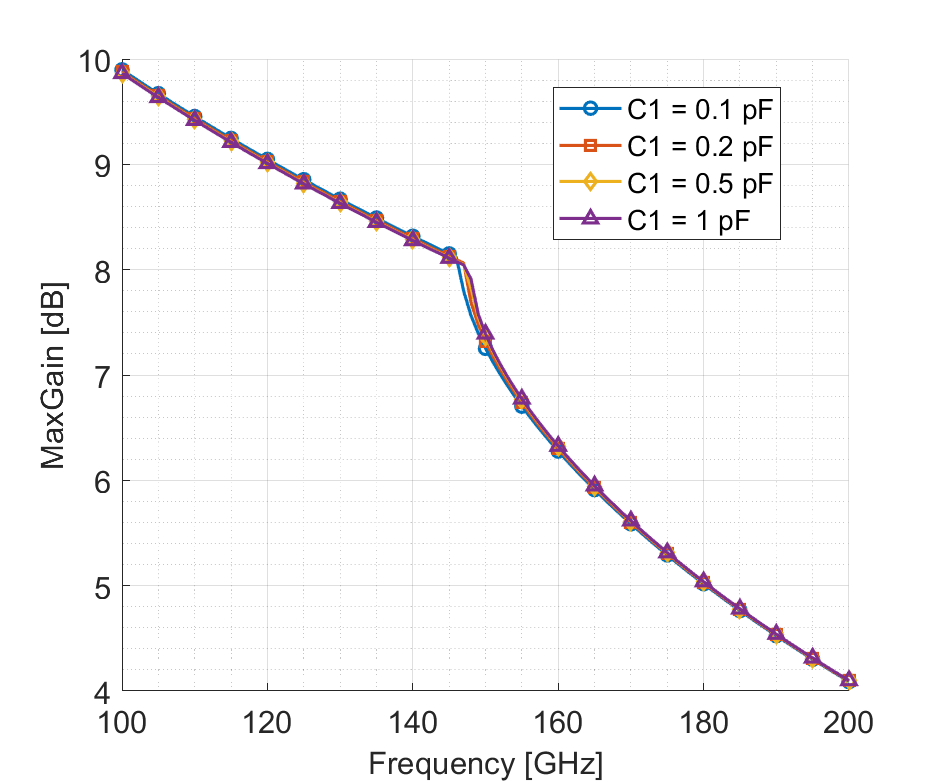
\includegraphics[width=0.5\linewidth]{Design_figures/Measurements/FirstStage/DiffBalun1_ExtractPar_SweepC1_conC2fermo_a1pF_S_MaxGain_MaxGain.png}
    \caption{Simulated maximum gain of the single-input, balanced-output differential amplifier schematic as a function of the swept $C_1$, with $C_2$ fixed at \SI{1}{\pico\farad}.}
    \label{fig:FirstStageSchematicMaxgainSweepC1}
\end{figure}\\
The capacitors had to be as small as possible without significantly affecting the amplitude balance. Therefore, a first sweep parameter simulation from \SI{1}{\pico\farad} down to \SI{0.1}{\pico\farad} was done with $C_2$ kept fixed at \SI{1}{\pico\farad}.
The MaxGain in Figure \ref{fig:FirstStageSchematicMaxgainSweepC1} remains unaffected during the sweep of $C_1$ as this parameter is mostly dependant by the transistor's Q1 and Q2 characteristics, such as the collector current and source and load terminations, as long as the current mirror works properly.
%
\begin{figure}[!hbt]
    \centering
    % --- Subfigure (a)
    \begin{subfigure}[b]{0.48\linewidth}
        \centering
        \begin{tikzpicture}
            \node[anchor=south west, inner sep=0] (imgA)
                {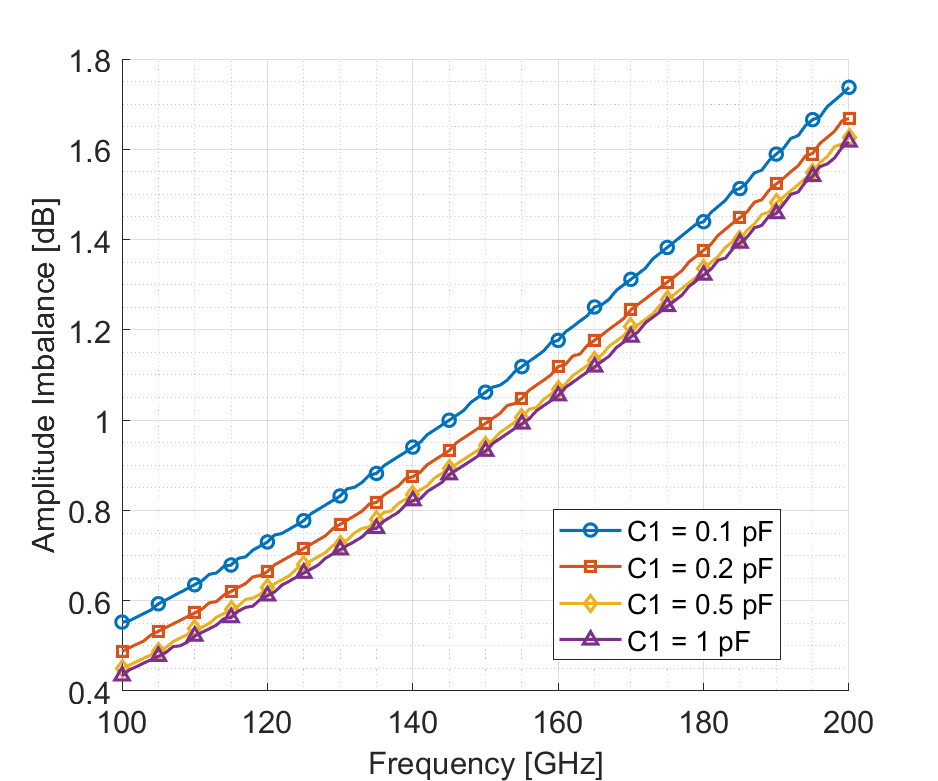
\includegraphics[width=\linewidth]{Design_figures/Measurements/FirstStage/DiffBalun1_ExtractPar_SweepC1_conC2fermo_a1pF_S_MaxGain_AmplitudeImbalance_dB.png}};
            % Ellisse e freccia
\begin{comment}
                \begin{scope}[x={(imgA.south east)}, y={(imgA.north west)}]
                \draw[thick, rotate around={0:(0.5,0.5)}]
                    (0.5,0.45) ellipse [x radius=0.045, y radius=0.1];
                \draw[-latex, thick](0.5,0.55)--++(0,0.08);
            \end{scope}
\end{comment}
        \end{tikzpicture}
        \caption{}
        \label{fig:FirstStageSchematicAmplitudeImbalanceSweepC1}
    \end{subfigure}
    \hfill
    % --- Subfigure (b)
    \begin{subfigure}[b]{0.48\linewidth}
        \centering
        \begin{tikzpicture}
            \node[anchor=south west, inner sep=0] (imgB)
                {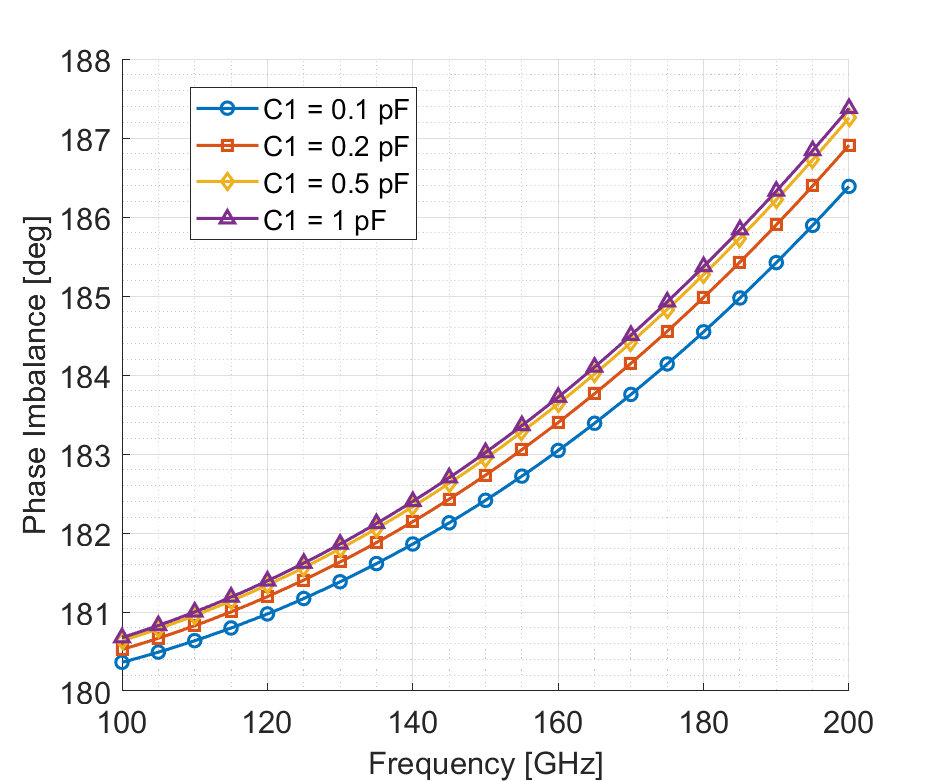
\includegraphics[width=\linewidth]{Design_figures/Measurements/FirstStage/DiffBalun1_ExtractPar_SweepC1_conC2fermo_a1pF_S_MaxGain_PhaseImbalance.png}};
            % Ellisse e freccia
\begin{comment}
                \begin{scope}[x={(imgB.south east)}, y={(imgB.north west)}]
                \draw[thick, rotate around={0:(0.5,0.5)}]
                    (0.5,0.375) ellipse [x radius=0.045, y radius=0.1];
                \draw[-latex, thick](0.5,0.275)--++(0,-0.08);
            \end{scope}
\end{comment}
        \end{tikzpicture}
        \caption{}
        \label{fig:FirstStageSchematicPhaseImbalanceSweepC1}
    \end{subfigure}

    \caption{
    Simulated results and comparison of the imbalances in the single-input balanced-output differential amplifier schematic: (a) amplitude imbalance and (b) phase imbalance as functions of the swept $C_1$, with $C_2$ fixed at \SI{1}{\pico\farad}.
    }
    \label{fig:FirstStageSchematicImbalanceSweepC1}
\end{figure}\\
Figure \ref{fig:FirstStageSchematicAmplitudeImbalanceSweepC1} shows that the $\Delta \varepsilon$ variation, although negligible, is inversely proportional to $C_1$ , while an opposite trend is observed for the $\Delta \phi$ in Figure \ref{fig:FirstStageSchematicPhaseImbalanceSweepC1}.
A possible explanation is to be associated to the current mirror output impedance: for at a given frequency, decreasing $C_1$ increases the input impedance at the base which, in turns, decreases the output impedance.
As the tail impedance has reduced, the input voltage at the CB, and so it's voltage gain, slightly dropped.
From the CE point of view, the degeneration emitter slightly lowers, and its gain increases. These two behaviours put together increase $\Delta \varepsilon$.
\begin{figure}[hbt!]
    \centering
    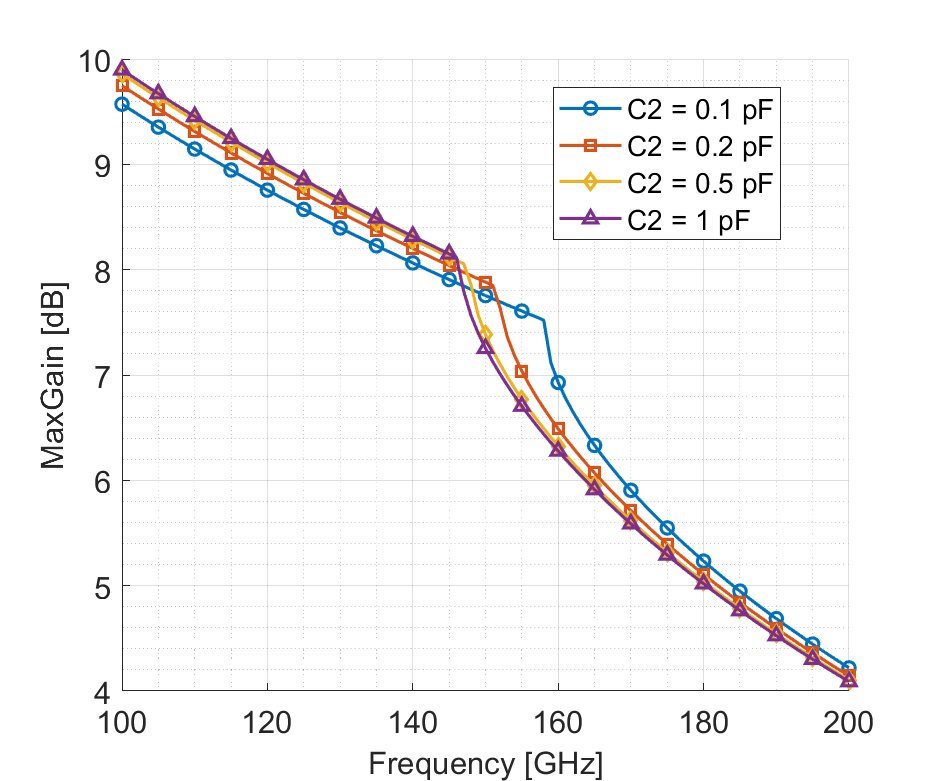
\includegraphics[width=0.5\linewidth]{Design_figures/Measurements/FirstStage/DiffBalun1_ExtractPar_SweepC2_conC1fermo_a0.1pF_S_MaxGain_MaxGain.png}
    \caption{Simulated MaxGain of the single-input balanced-output differential amplifier schematic as a function of the swept $C_2$, with $C_1$ fixed at \SI{0.1}{\pico\farad}.}
    \label{fig:FirstStageSchematicMaxGainSweepC2}
\end{figure}
\\
A sweep-parameter simulation was performed on capacitor $C_2$, located at the base of Q2, from \SI{1}{\pico\farad} down to \SI{0.1}{\pico\farad}, while $C_1$ was kept fixed at \SI{0.1}{\pico\farad}.
The variation of the shunt capacitor $C_2$ causes a slight variation in the MaxGain,  Figure \ref{fig:FirstStageSchematicMaxGainSweepC2}, due to changes in the output impedance of Q3.
Furthermore, the analysis made for $C_1$ can be applied to describe the changes in $\Delta \varepsilon$ and $\Delta \phi$, shown in Figures \ref{fig:FirstStageSchematicAmplitudeImbalanceSweepC2} and \ref{fig:FirstStageSchematicPhaseImbalanceSweepC2}, respectively.
Also, with the reduction of $C_2$, the emitter impedance decreases, affecting the CE emitter degeneration by means of the parallel combination of the mirror $Z_{tail}$ and the $R_{CEeq}$ seen by the CB.


\begin{figure}[hbt!]
    \centering
    % --- Subfigure (a)
    \begin{subfigure}[b]{0.48\linewidth}
        \centering
        \vspace{0pt}
        \begin{tikzpicture}
            \node[anchor=south west, inner sep=0] (imgA)
                {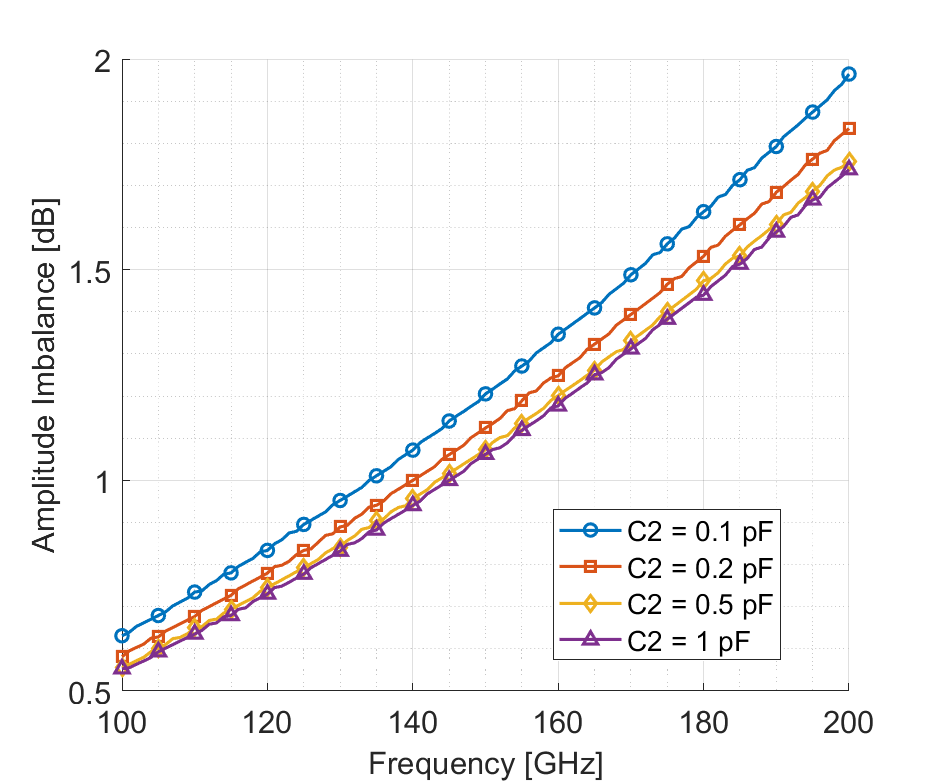
\includegraphics[width=\linewidth]{Design_figures/Measurements/FirstStage/DiffBalun1_ExtractPar_SweepC2_conC1fermo_a0.1pF_S_MaxGain_AmplitudeImbalance_dB.png}};
            % Esempio: Ellisse e freccia sopra
            \begin{comment}
                \begin{scope}[x={(imgA.south east)}, y={(imgA.north west)}]
                \draw[thick, rotate around={0:(0.5,0.5)}]
                    (0.5,0.45) ellipse [x radius=0.045, y radius=0.1];
                \draw[-latex, thick](0.5,0.55)--++(0,0.08);
            \end{scope}
            \end{comment}
        \end{tikzpicture}
        \caption{}
        \label{fig:FirstStageSchematicAmplitudeImbalanceSweepC2}
    \end{subfigure}
    \hfill
    % --- Subfigure (b)
    \begin{subfigure}[b]{0.48\linewidth}
        \centering
        \vspace{0pt}
        \begin{tikzpicture}
            \node[anchor=south west, inner sep=0] (imgB)
                {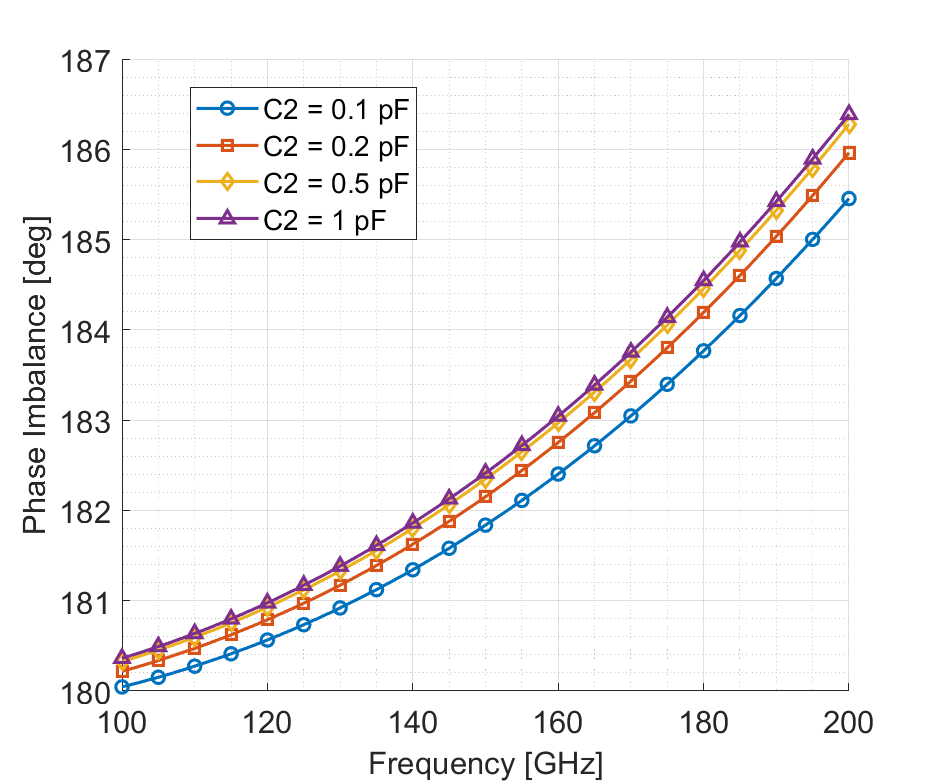
\includegraphics[width=\linewidth]{Design_figures/Measurements/FirstStage/DiffBalun1_ExtractPar_SweepC2_conC1fermo_a0.1pF_S_MaxGain_PhaseImbalance.png}};
            % Esempio: Ellisse e freccia sopra
\begin{comment}
                \begin{scope}[x={(imgB.south east)}, y={(imgB.north west)}]
                \draw[thick, rotate around={0:(0.5,0.5)}]
                    (0.5,0.35) ellipse [x radius=0.045, y radius=0.1];
                \draw[-latex, thick](0.5,0.25)--++(0,-0.08);
            \end{scope}
\end{comment}
        \end{tikzpicture}
        \caption{}
        \label{fig:FirstStageSchematicPhaseImbalanceSweepC2}
    \end{subfigure}

    \caption{Simulated results and comparison of the imbalances in the single-input balanced-output differential amplifier schematic: (a) amplitude imbalance and (b) phase imbalance as functions of the swept $C_2$, with $C_1$ fixed at \SI{0.1}{\pico\farad}.}
    \label{fig:FirstStageSchematicImbalanceSweepC2}
\end{figure}

%A further estimation of the inductor parasitics of transmission lines made in conjunction with the layout are shown in the schematic in figure XX and the final results in FIgure XX YY and ZZ.
%\begin{figure}
%    \centering
%    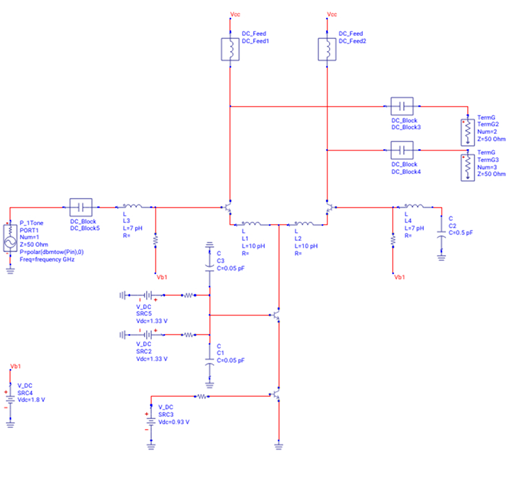
\includegraphics[width=1\linewidth]{Design_figures/Schematics/FirstStageApproxParam.png}
%    \caption{Caption}
%    \label{fig:placeholder}
%\end{figure}

%%%%%%%%%%%%%%%%%%%%%%%%%%%%%%%%%%%%%%%%%%%%%%%%%%%%%%%%%%%%%%%%%%%
%
\clearpage
\subsubsection{Design of the Second Stage}
%
%%%%%%%%%%%%%%%%%%%%%%%%%%%%%%%%%%%%%%%%%%%%%%%%%%%%%%%%%%%%%%%%%%%
The differential amplifier double-input balanced-output shown in Figure \ref{fig:SchematicSecondStage} is the second stage of the design and its purpose is to improve the amplitude and phase balance by rejecting the common mode signal component coming from the previous stage.
\begin{figure}[hbt!]
    \centering
    \begin{circuitikz}[scale=0.85, transform shape]
    \draw (0,0) node[npn, xscale=1, anchor=B] (Q1)
    {\shortstack{$Q5$ \\ 2}};
    %metto metà sinistra dell'emettitore
    \draw (Q1.E)--++(0,-0.35)--++(1.1,0) coordinate(e);
    %metto metà destra dell'emettitore e Q2
    \draw(e)--++(1.1,0) --++(0,+0.35) node[npn, xscale=-1, anchor=E] (Q2){\ctikzflipx{\shortstack{$Q6$ \\ 2}}};
    %disegno current mirror
    \draw (e) to [short,*-]++(0,-0.25) node[npn, xscale=1, anchor=C] (Q3)
    {\shortstack{$Q7$ \\ 2}};
    \draw (Q3.E) --++(0,-0.5) node[npn, xscale=1, anchor=C] (Q4){\shortstack{$Q8$ \\ 2}} ;
    \draw (Q4.E) --++(0,-0.15) node[tlground]{};
    
    %inserisco le resistenze bias AC block
    %biasin a Q1
    \draw (Q1.B)--++(-0.85,0) coordinate (in1)
    to [R,l=$\mathrm{R}_5$]++(0,1.5)
    to [open]++(-0.35,0) --  node[anchor=south] {$\mathrm{V}_{\mathrm{CC}}$} ++(0.7,0);
    %biasing a Q2
    \draw (Q2.B)--++(0.85,0) coordinate (in2)
    to [R,l=$\mathrm{R}_6$]++(0,1.5) to [open]++(-0.35,0) --  node[anchor=south] {$\mathrm{V}_{\mathrm{CC}}$} ++(0.7,0);
    %biasing current mirror Q3
    \draw (Q3.B) to [short]++(-0.15,0) coordinate (in3);
    \draw (in3)to [short,*-]++(-0.25,0) to [R,l_=$\mathrm{R}_7$]++(-2,0) to [short,-o]++(-0.25,0) node[left]{$\mathrm{V}_{\mathrm{B2}}$};
    \draw (in3) to [C,l_=$C_1$]++(0,-1.25)node[tlground]{};
    %biasing current mirror Q4
    \draw (Q4.B) to [R,l_=$\mathrm{R}_8$]++(-1.25,0) to [short,-o]++(-0.25,0) node[left]{$\mathrm{V}_{\mathrm{B1}}$};
    %inserisco input a base Q1
    \draw (in1) to [C,*-o] ++(-1.6,0) coordinate(dc1)node[left]{$V_{in+}$};
    %inserisco capacità a base Q2
    \draw (in2)to [open,-*]++(-0.5,0) to [short]++(0,-1.4)to[short]++(-5.1,0) to [C,-o] ++(-1.6,0) coordinate(dc2)node[left]{$V_{in-}$};
    
    \draw (dc1) to [open]++(0.275,-0.375) rectangle++(1.05,0.75);
    \draw (dc2) to [open]++(0.275,-0.375) rectangle++(1.05,0.75);
    
    %disegno collettore Q1
    \draw (Q1.C) --++ (0,1) coordinate(c1) to [L]++(0,2.15) to [open]++(-0.35,0) --  node[anchor=south] {$\mathrm{V}_{\mathrm{CC}}$} ++(0.7,0);
    \draw (c1) to [short,*-o]++(0.5,0)node[above]{+};
    
    \draw (Q2.C) --++ (0,1) coordinate(c2) to [L]++(0,2.15) to [open]++(-0.35,0) --  node[anchor=south] {$\mathrm{V}_{\mathrm{CC}}$} ++(0.7,0);
    \draw (c2) to [short,*-o]++(-0.5,0)node[above]{-};
    
    \node[draw, fill=white, rounded corners] at (8,2) {
      $\begin{array}{r@{\,}c@{\,}l}
      \text{V}_\text{CC}   &=& \SI{1.8}{\volt} \\
      \text{V}_\text{B1}   &=& \SI{0.93}{\volt} \\
      \text{V}_\text{B2}   &=& \SI{1.33}{\volt} \\
      \text{R}_5, \text{R}_6 &=& \SI{2}{\kilo\ohm} \\
      \text{R}_7, \text{R}_8 &=& \SI{2}{\kilo\ohm} \\
      \text{C}_1      &=& \SI{0.1}{\pico\farad}
      \end{array}$
    };

    %riquadri
    \draw (0.425,2.23)rectangle++(0.75,1.25);
    \draw (0.425+2.2,2.23)rectangle++(0.75,1.25);
\end{circuitikz}
\caption{Schematic of the differential amplifier with differential input and balanced output.}
\label{fig:SchematicSecondStage}
\end{figure}

Because the design of the second stage is an exact replica of the first one, except for the input routing, it will not be discussed thoroughly in order to avoid redundancies with what was previously explained in Section~\ref{subsubsec:Design of the First Stage}.

\begin{figure}[hbt!]
    \centering
    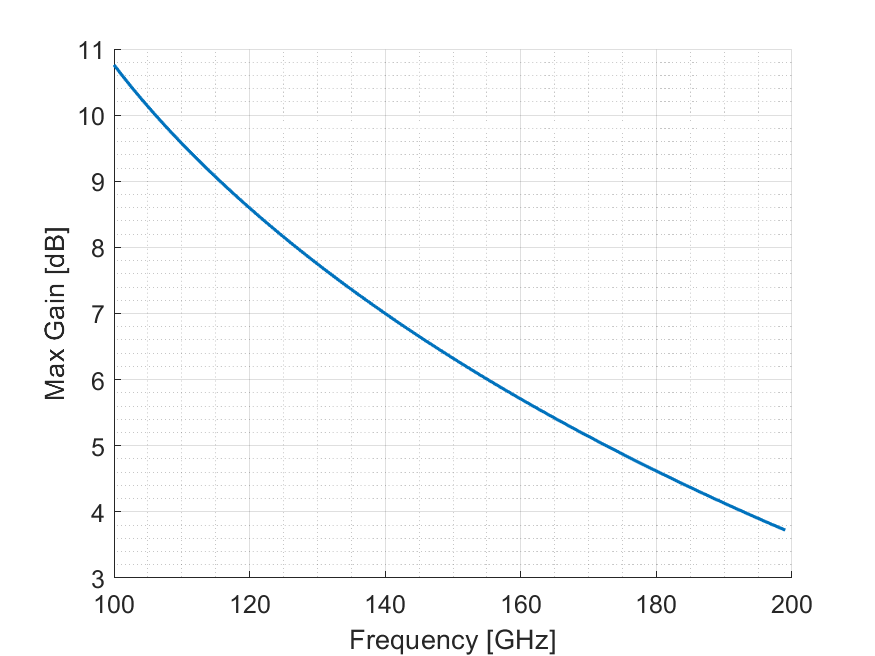
\includegraphics[width=0.5\linewidth]{Design_figures/Measurements/SecondStage/DiffAmplifier1_ExtractPar_C1setTo_0.1pF_S_MaxGain_MaxGain.png}
    \caption{Simulated MaxGain of the double-input balanced-output differential amplifier schematic for $C_1 = \SI{0.1}{\pico\farad}$.}
    \label{fig:SchematicSecondStage_measureMaxGain}
\end{figure}
Figure~\ref{fig:SchematicSecondStage_measureMaxGain} shows the ideally obtainable MaxGain, which goes from \SI{11}{\decibel} to \SI{4}{\decibel} with the same trend over frequency.\\
Given the differential nature of this stage and the ideal differential input, the amplitude and phase imbalance plots were omitted, as they did not provide any additional information other than \SI{0}{\decibel} for $\Delta \varepsilon$ and \SI{180}{\degree} for $\Delta \phi$ across all frequencies.

%%%%%%%%%%%%%%%%%%%%%%%%%%%%%%%%%%%%%%%%%%%%%%%%%%%%%%%%%%%%%%%%%%%
%

\subsubsection{Design of the Third Stage}
%
%%%%%%%%%%%%%%%%%%%%%%%%%%%%%%%%%%%%%%%%%%%%%%%%%%%%%%%%%%%%%%%%%%%
The stages described so far weren't designed to boost the gain, so an amplifier block was necessary.
In this regard, any amplifier design could be used as long as it fits the requirements defined by the voltage supply, efficiency, and by it's possibility to be as symmetric as possible.
For this project, a first analysis of the basic transistor configurations was done to check which one could give the MaxGain in the D band. 

\begin{figure}[hbt!]
    \centering
    
    \begin{subfigure}{0.5\textwidth}
        \centering
        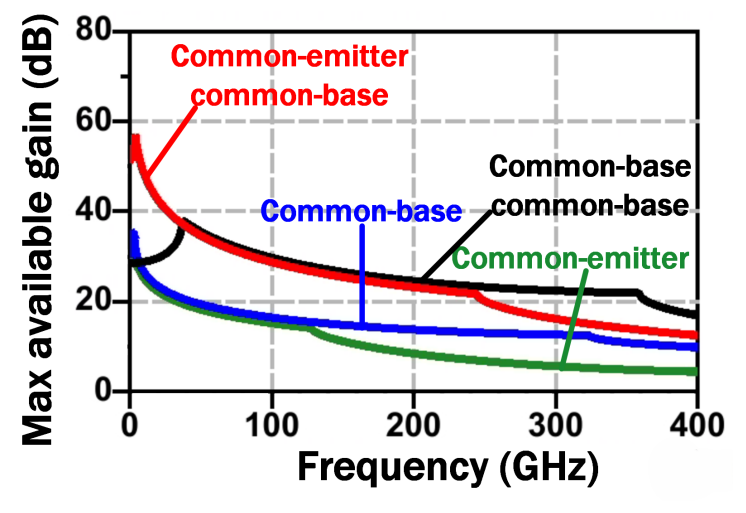
\includegraphics[width=\linewidth]{Design_figures/AmplifiersMaxGain_AnielloPaper.png}
        \caption{Maximum available gain for different amplifier topologies, from \cite{Considerations and Methods on the Design of sub-THz Amplifiers in SiGe BiCMOS Technology}}
        \label{fig:AmplifiersMaxGain_AnielloPaper}
    \end{subfigure}
    \hfill
    \begin{subfigure}{0.46\textwidth}
        \centering
        \begin{circuitikz}[scale=0.75,transform shape]
        
        % Transistor
        \draw (0,0) node[npn, anchor=B] (Q1)
        {\shortstack{$Q$}};
        
        % Base branch
        \draw (Q1.B) to [short]++(-0.25,0) coordinate (vb1)--++(-0.25,0);
        \draw (vb1) --++(-0.25,0) coordinate(b1)
              to [L,mirror]++(-2,0) 
              to [short,-o]++(-0.25,0) node[left]{$V_\mathrm{B}$};
        \draw (vb1) to [C,l_=$C$,*-]++(0,-1.35) node[tlground]{};
        
        % Collector branch
        \draw (Q1.C) --++ (0,0.25) coordinate(c1)
              to [L,mirror]++(0,2)
              to [open]++(-0.35,0) -- node[anchor=south] {$\mathrm{V}_\mathrm{CC}$} ++(0.7,0);
        \draw (c1) to [C,*-o]++(2,0) node[right]{$v_\mathrm{out}$};
        
        % Emitter branch
        \draw (Q1.E) --++(0,-0.75) coordinate (in1);
        \draw (in1) --++ (0,-0.75) coordinate(e1)
              to [L]++(0,-2.3) node[tlground]{};
        \draw (e1) to [C,*-o]++(-2,0) node[left]{$v_\mathrm{in}$};
        
        % Highlight rectangles
        \draw (c1) to [open]++(-0.35,0.35) rectangle++(0.75,1.25);
        \draw (c1) to [open]++(0.5,-0.425) rectangle++(1,0.85);
        \draw (e1) to [open]++(-0.35,-0.5) rectangle++(0.75,-1.25);
        \draw (e1) to [open]++(-0.5,-0.425) rectangle++(-1,0.85);
        \draw (b1) to [open]++(-0.35,-0.35) rectangle++(-1.25,0.75);
        
        \end{circuitikz}
        \caption{Schematic of a CB amplifier}
        \label{fig:BJTCB_single_stage}
    \end{subfigure}
    \caption{Comparison of the maximum available gain for different amplifier topologies and schematic of the common-base amplifier topology.}
\end{figure}
To help with the decision, paper \cite{Considerations and Methods on the Design of sub-THz Amplifiers in SiGe BiCMOS Technology}, from which Figure \ref{fig:AmplifiersMaxGain_AnielloPaper} was consulted. The figure
compares four amplifier topologies and it is possible to observe that a CE configuration performances are surclassed by other topologies after \SI{150}{\giga \hertz} and giving at best \SI{8}{\decibel} at \SI{200}{\giga \hertz}.
Furthermore, from the same paper it is possible to conclude that a single stage CB amplifier with 8 emitter fingers properly biased for MaxGain is capable of achieving \SI{15}{\decibel} at \SI{200}{\giga \hertz}, indicating that increasing the number of fingers from an initial value of 2, as in previous stages, to a greater one is a potential solution to the lack of the overall gain at higher frequencies.

Figure \ref{fig:BJTCB_single_stage} shows the basic circuit investigated in this section.
The lack of data does not allow a proper evaluation of the causes of some changes, but an estimate can still be made.
The base voltage is initially set to \SI{0.87}{\volt}, the collector current is fixed at \SI{7.3}{\milli\ampere} and the biasing network consists of an ideal DC-feed inductor.
Replacing the emitter DC feed with an ideal inductor does not change the results, as long as the other DC components are completely ideal, as shown in Figure \ref{fig:CBamplifier_ExtractPar_SweepInductor_and_SweepFinger_S_MaxGain_MaxGain}. 
\begin{comment}
    The figure compares the MaxGain of the 6-finger CB amplifier with that of a 2-finger alternative, whose displayed performance is better than the first one because \SI{7}{\milli\ampere} is close to its maximum collector current.
\end{comment}
%
\begin{figure}[hbt!]
    \centering
    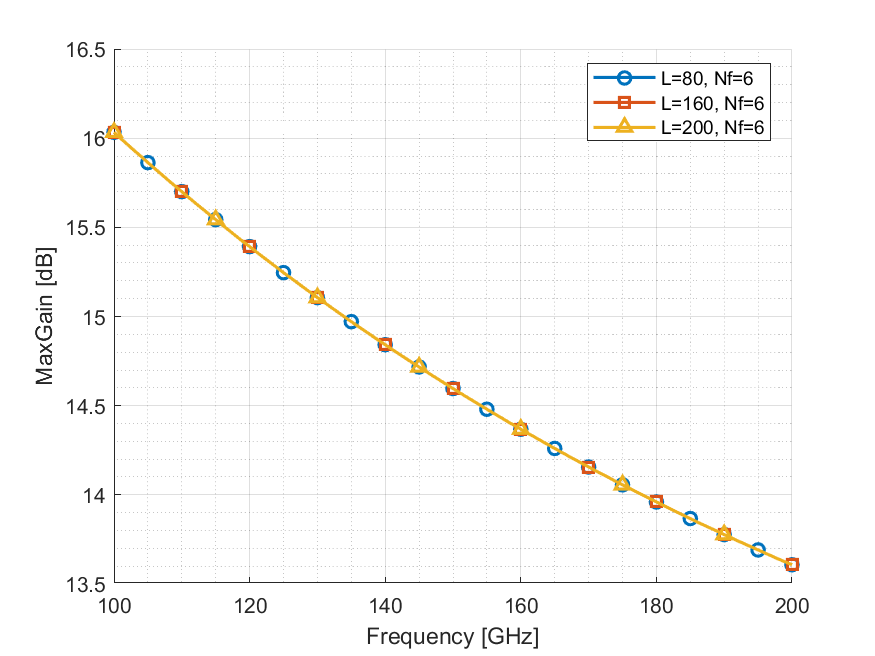
\includegraphics[width=0.55\linewidth]{Design_figures/Measurements/ThirdStage/CBamplifier_ExtractPar_SweepInductor_and_SweepFinger_S_MaxGain_MaxGain.png}
    \caption{Simulated maximum gain for different emitter DC-feed values in the 6-finger CB amplifier.}
    \label{fig:CBamplifier_ExtractPar_SweepInductor_and_SweepFinger_S_MaxGain_MaxGain}
\end{figure}
%
\\At this point multiple changes were applied starting from the topology. Two single stage CB amplifiers were condensed in one single core with a symmetrical design, shown in Figure \ref{fig:SchematicSymmetricThirdStage}.

\begin{figure}[hbt!]
    \centering
    \begin{circuitikz}[scale=0.85, transform shape]
    \draw (0,0) node[npn, yscale=-1, anchor=B] (Q1)
    {\reflectbox{\rotatebox{180}{\shortstack{$Q9$ \\ 6}}}};
    %inserisco ramo base di Q1
    \draw (Q1.B) to [short]++(-0.5,0) coordinate (vb1);
    \draw (vb1) to [R,l_=$\mathrm{R}_9$,*-o]++(-2.3,0) node[left]{$\mathrm{V}_{\mathrm{B}}$};
    \draw (vb1) --++(0,-2) coordinate (x);
    \draw (x) to [C,l_=$C_3$,*-]++(-2,0)node[rotate=-90, tlground]{};
    
    %inserisco ramo collettore Q1
    \draw (Q1.C) --++ (0,-0.25) to [short]++(1.5,0)coordinate(c1) to [L,*-,mirror]++(0,2) to [open]++(-0.35,0) --  node[anchor=south] {$\mathrm{V}_{\mathrm{CC}}$} ++(0.7,0);
    \draw (c1) --++(0.05,0) to [C,-o]++(2,0) node[right]{$v_\mathrm{out+}$};
    
    %inserisco ramo emettitore di Q1
    \draw (Q1.E) --++(0,0) coordinate (in1);
    \draw (in1) --++ (0,0.75) coordinate(e1) to [L,mirror]++(0,2.3) node[yscale=-1, tlground]{};
    \draw (e1) to [C,*-o]++(-2,0) node[left]{$V_{in+}$};
    
    %ricreo il circuito mirrored
    \begin{scope}[shift={(0,-4)}, yscale=-1, transform shape]
    \draw (0,0) node[npn, yscale=-1, anchor=B] (Q1)
    {\shortstack{$Q10$ \\ 6}};
    %inserisco ramo base di Q1
    \draw (Q1.B) to [short]++(-0.5,0) coordinate (vb1);
    \draw (vb1) to [R, l=\reflectbox{\rotatebox{180}{$\mathrm{R}_{10}$}},*-o, label distance=-6.5mm]++(-2.3,0) node[left]{\reflectbox{\rotatebox{180}{$\mathrm{V}_{\mathrm{B}}$}}};
    \draw (vb1) --++(0,-2);
    
    %inserisco ramo collettore Q1
    \draw (Q1.C) --++ (0,-0.25) to [short]++(1.5,0)coordinate(c2) to [L,*-,mirror]++(0,2) to [open]++(-0.35,0) --  node[anchor=south] {\reflectbox{\rotatebox{180}{$\mathrm{V}_{\mathrm{CC}}$}}} ++(0.7,0);
    \draw (c2) --++(0.05,0) to [C,-o]++(2,0) node[right]{\reflectbox{\rotatebox{180}{$v_\mathrm{out-}$}}};
    
    %inserisco ramo emettitore di Q1
    \draw (Q1.E) --++(0,0) coordinate (in1);
    \draw (in1) --++ (0,0.75) coordinate(e2) to [L,mirror]++(0,2.3) node[yscale=-1, tlground]{};
    \draw (e2) to [C,*-o]++(-2,0) node[left]{\reflectbox{\rotatebox{180}{$v_{in-}$}}};
    \end{scope}

      \node[draw, fill=white, rounded corners] at (7,2) {
      $\begin{array}{r@{\,}c@{\,}l}
      \text{V}_\text{CC}   &=& \SI{1.8}{\volt} \\
      \text{V}_\text{B}   &=& \SI{0.9}{\volt} \\
      \text{R}_9, \text{R}_{10} &=& \SI{2}{\kilo\ohm} \\
      \text{C}_3      &=& \SI{0.25}{\pico\farad}
      \end{array}$
    };
  %aggiungo node invisibile a sinistra per centrare il circuito 
  \node[ fill=white, rounded corners, align=center] at (-6.5,2) {
  };
    %label L1 e L2
    \draw (e1)to [open]++(0.75,1.15) node[]{$L1$};
    \draw (e2)to [open]++(0.75,-1.15) node[]{$L2$};
    %riquadri
    \draw (c1) to [open]++(-0.35,0.35)rectangle++(0.75,1.25);
    \draw (c1) --++(0.05,0) to [open]++(0.5,-0.425) rectangle++(1,0.85);
    
    \draw (c2) to [open]++(-0.35,-0.35)rectangle++(0.75,-1.25);
    \draw (c2) --++(0.05,0) to [open]++(0.5,-0.425) rectangle++(1,0.85);
    
    \draw (e1) to [open]++(-0.35,0.5) rectangle ++(0.75,1.25);
    \draw (e2) to [open]++(-0.35,-0.5) rectangle ++(0.75,-1.25);
    
    \draw (e1) to [open]++(-0.5,-0.425) rectangle ++(-1,0.85);
    \draw (e2) to [open]++(-0.5,-0.425) rectangle ++(-1,0.85);

   \draw[color=red,dashed, thick]
    (x) --++(0,0.6)  arc[start angle=0, end angle=90, radius=3mm] % punto di partenza (a destra e leggermente sopra)
    -- ++(-1.85,0) arc[start angle=90, end angle=185, radius=3mm]
    -- ++(0,-1.1) arc[start angle=185, end angle=270, radius=3mm]
    -- ++(1.85,0) arc[start angle=270, end angle=360, radius=3mm] -| (x);

    \draw[color=red,dashed, thick] (x) to [open]++(0,0.7)--++(-2.7+0.25,-1.3);
\end{circuitikz}
\caption{Schematic of two common-base amplifiers in a symmetric configuration.}
\label{fig:SchematicSymmetricThirdStage}
\end{figure}
%
The DC-feed component at the base was replaced with a \SI{2}{\kilo\ohm} resistor, while the DC feed at the emitters remained unchanged. Furthermore, the base voltage was increased to \SI{0.9}{\volt}, while the collector current remained at \SI{7.3}{\milli\ampere}. Under these conditions, the current density of Q9 and Q10 is close to \SI{12.5}{\milli\ampere\per\micro\meter\squared}. As a result, $f_T$ and $f_{\mathrm{MAX}}$, shown in Figure~\ref{fig:FtFmaxSG13G3}, are reduced to about \SI{390}{\giga\hertz} and \SI{550}{\giga\hertz}, respectively. This choice was mainly made to keep the stage efficient.\\
A worsening of the MaxGain can be seen in Figure~\ref{fig:CBamplifier2_ExtractPar_Symmetric_SweepBias_SweepInductor_and_SweepFinger_S_MaxGain_MaxGain_merged}: it starts at about \SI{12.5}{\decibel} and decreases to about \SI{7}{\decibel} over the frequency range.
Moreover, replacing the emitter DC-feed chokes L1 and L2 with ideal inductors further reduces the MaxGain. Under these conditions, a sweep of these inductors was carried out to find a value that does not significantly degrade the performance, showing that a value between \SI{80}{\pico\henry} and \SI{200}{\pico\henry} would have been preferable.
%which is three times greater than the current in use.
\\
\begin{figure}[hbt!]
    \centering
    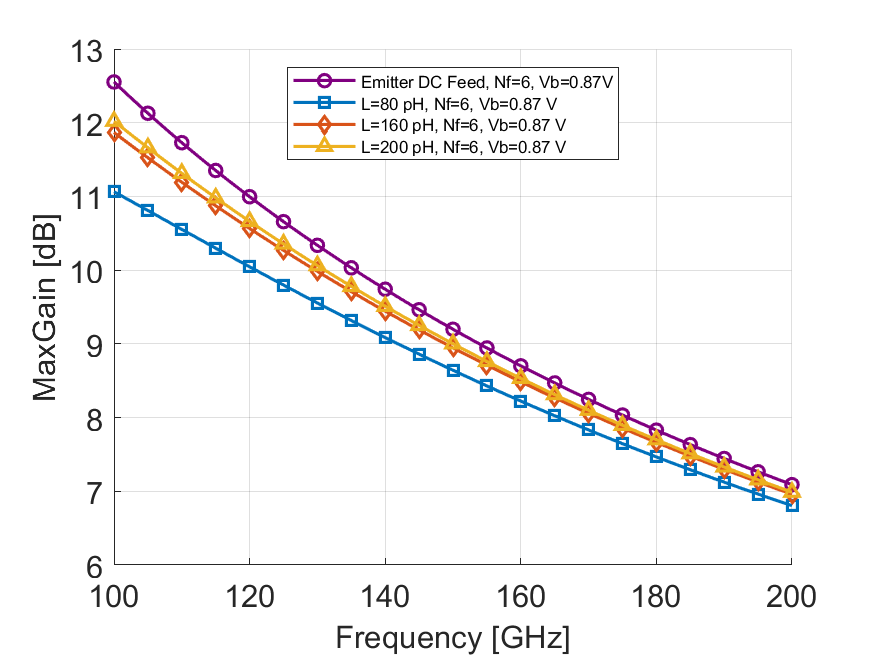
\includegraphics[width=0.55\linewidth]{Design_figures/Measurements/ThirdStage/CBamplifier2_ExtractPar_Symmetric_SweepBias_SweepInductor_and_SweepFinger_S_MaxGain_MaxGain_merged.png}
    \caption{Simulated maximum gain of the CB amplifier schematic as a function of the DC-feed inductors.}
    \label{fig:CBamplifier2_ExtractPar_Symmetric_SweepBias_SweepInductor_and_SweepFinger_S_MaxGain_MaxGain_merged}
\end{figure}
The layout implementation will not use the capacitor for reasons that will be explained in Section \ref{subsubsec:Layout of the third stage}. For completeness, the circuit is shown as originally intended, so as to also allow alternatives and conclusions to be drawn.


%The results were not as good as described in the single stage CB amplifier. In the symmetric configuration, the Max gain measurement got degraded to a level of \SI{8}{\decibel} at \SI{200}{\giga \hertz}, almost half of what it was supposed to give.\\
\begin{comment}
\begin{figure}[hbt!]
    \centering
     \begin{tikzpicture}[scale=0.75,transform shape]
            \node[anchor=south west, inner sep=0] (imgA)
                {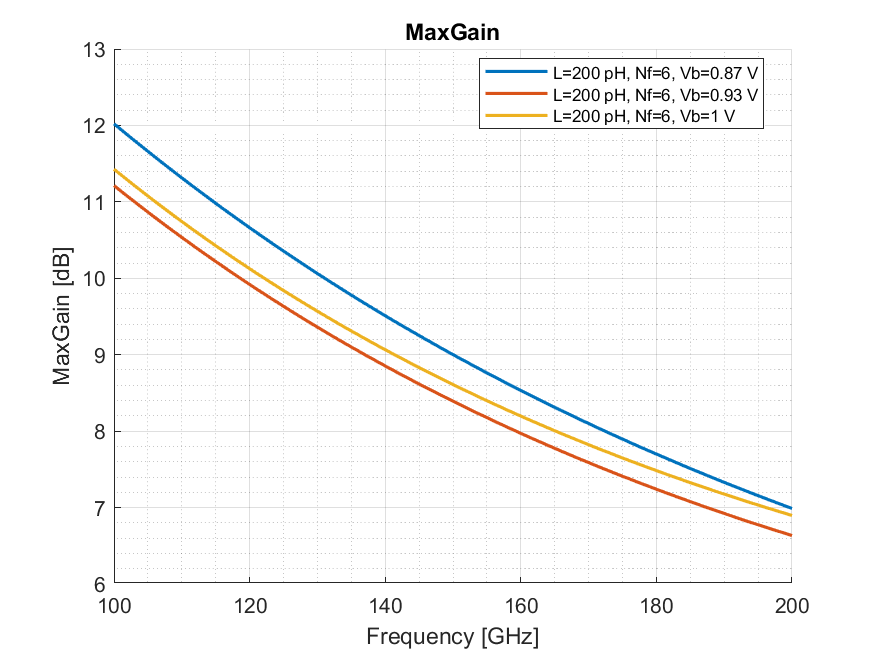
\includegraphics[width=\linewidth]{Design_figures/Measurements/ThirdStage/CBamplifier2_ExtractPar_Symmetric_SweepBias_Finger6_MaxGain.png}};
        \end{tikzpicture}
    \caption{Simulated results and MaxGain comparison symmetric CB amplifiers schematic as a function of the swept voltage}
    \label{fig:placeholder}
\end{figure}
\end{comment}
%
%\textcolor{red}{Come sarebbe stato il maxgain EM 3 stadi con la capacità? una foto la si vede in pptx Differenziale slide 86.. da 20dB a 15dB in tutta la banda }\\
%\textcolor{blue}{Perchè ho tolto la capacità? quale era l'obiettivo? è stato fatto quasi all'ultimo momento; l'obiettivo era cercare un modo per migliorare l'impedenza in uscita dall'amplificatore CB. Con la Capacità le impedenze si aggiravano intorno ai 8 ohm. senza la capacità la port2 saliva a 34 ohm mentre quella di Port3 saliva a 25. valori in pptx Matchin network slide 60 => questo però compara il primo caso con l'induttore ideale.. forse i risultati più veritieri sono tra slide 10 e 12 }


\cleardoublepage



\begin{comment}
\begin{circuitikz}
    \draw (0,0) node[npn, xscale=1, anchor=B] (Q1)
    {\shortstack{$Q1$ \\ 6}};
    %inserisco ramo base di Q1
    \draw (Q1.B) to [short]++(-0.5,0) coordinate (vb1);
    \draw (vb1)--++(-0.25,0) to [R,l_=$R_{1}$]++(-1.75,0) to [short,-o]++(-0.25,0) node[left]{$V_{b}$};
    \draw (vb1) to [C,l_=$C$]++(0,-1.25)node[tlground]{};
    
    %inserisco ramo collettore Q1
    \draw (Q1.C) --++ (0,1) coordinate(c1) to [L,mirror]++(0,2) to [open]++(-0.35,0) --  node[anchor=south] {Vcc} ++(0.7,0);
    \draw (c1) to [short,*-]++(2,0);
    
    %inserisco ramo emettitore di Q1
    \draw (Q1.E) --++(0,-0.75) coordinate (in1);
    \draw (in1) --++ (0,-0.75) coordinate(e1) to [L]++(0,-2.3) node[tlground]{};
    \draw (e1) to [C,*-]++(-2,0) node[left]{Vin};

    %valori
    \node at (-3,4) {\parbox{2cm}{
    \centering 
    Vcc=$1.8$V \\ 
    Vb1=$0.92$V \\
    Vb2=$1.33$V \\
    $R_1$,$R_2$,$R_3$,$R_4$=\SI{2}{\kohm}
    $C_1$=\SI{0.1}{\pF}
    $C_2$=\SI{0.5}{\pF}
    }};

    %riquadri
    %riquadri
    \draw (c1) to [open]++(-0.35,0.35)rectangle++(0.75,1.25);

    \draw (e1) to [open]++(-0.35,-0.5) rectangle ++(0.75,-1.25);
    \draw (e1) to [open]++(-0.5,-0.425) rectangle ++(-1,0.85);


\end{circuitikz}
\end{comment}